\section{Machine learning}
    
    This section serves as an introduction to the machine learning algorithms worked with in this project. Logistic regression, support vector machines and neural networks are the algorithms used. They are presented to give an intuitive understanding of how they work. What is presented in this section is mostly based on \cite{Hastie}. In addition a lot of the intuitive understanding comes from Andrew Ng's online courses, \cite{machinlearning} and \cite{deepLearning}.
    
    The methods used in this project have been chosen because they span the machine learning universe from simple to advanced. Firstly, this is done to ensure that one does not use unnecessary complicated methods. If simpler methods are good enough, they might be easier to interpret than the more complex ones. Secondly, more complicated methods will most likely give longer training and run-time. Two Python libraries are used for the analysis. Scikit-learn \cite{scikit-learn}, \cite{scikit-web} for logistic regression and support vector machines, and Keras \cite{chollet2015keras} for neural networks. There are a number of different libraries available, but these are chosen due to their ease of use, and the fact that Keras has an API that allows it to be used through Scikit-learn. This means that a lot of code can be reused when using the two libraries. 
        
    
    \subsection{Terminology}
        To simplify the further reading, some of the terminology used further is explained here. 
        
        \begin{itemize}
            \item ML, short of machine learning
            \item A variable is in ML referred to as a feature
            \item One data sample is also known as a feature vector, av vector holding the value of each of the features for this variable
            \item A class, is one of the different groups a feature vector can belong to.
            \item In classification you have a limited number of possible classes a feature vector can belong to. If you don't have a limited number of classes, regression  can be used to estimate the value.  
            \item For classification, a label tells you which class a feature vector belongs to.
            \item NN, short for neural network
            \item SVM, short for support vector machine
            \item LR, short for logistic regression
            \item Objective/scoring function, function used by the algorithm to optimize the results. 
        \end{itemize}
    
    \subsection{Supervised vs unsupervised algorithms}
        There are two main classes of machine learning algorithms, supervised and unsupervised. In supervised algorithms, you have labeled data. This means that you have data from the different types of scenarios you want to analyze. Say you want to build a machine learning algorithm that estimates the value of your used car. Then you need to collect information of already sold cars, the price they were sold for and a set of car features. Examples of useful features would be engine size, mileage, color, seats, drive type etc. Now you have a labeled dataset where each car with its features have a labeled price. You can then use supervised learning to train a classifier based on the data set, which you then can use to estimate the price of your car. In unsupervised learning, the price of the sold cars are unknown. What can be done here, is to analyze the data and look for unknown common structures. It is basically a grouping algorithm, that groups similar feature vectors together, which then later can be used to classify new feature vectors. 
        
        Supervised algorithms can again be split into two different sections. Regression or classification. In regression you have a continuous output range, as with the car example above. Then you want your algorithm to give you an estimate of the car price with an exact value. In classification however, you have a set of classes you want to classify all your data with. One might not need an accurate prediction of the price of a car, instead an estimated price range might be good enough.
        
    
    \subsection{The different algorithms}
        
            
            Note that the mathematical explanation of the algorithms are general approaches to explain how they work, the algorithms used does not necessarily use the exact same equations, but the general idea is similar. 
        
        \subsubsection{Linear regression}
            Linear regression serves as a good introduction to how machine learning works. It is also the basis for Logistic regression which is used in this analysis. Linear regression finds the best linear solution to your estimation problem. Based on you input features and labels for the data points, a linear function is fitted to the data. This is done by minimizing 
            \begin{align}
                J(\bm\theta) = \frac{1}{2m} \sum_{i=1}^{m}(h_\theta(\bm x^i) - y^i)^2.
                \label{linreg:cost}
            \end{align}
            
            You want the prediction 
            \begin{align}
                h_{\theta}(\bm x) = \theta_0 + \theta_{1}x_1 + \theta_{2}x_2 + ...+ \theta_{n}x_n,
                \label{linreg:h}
            \end{align}
            
            to be as close to $y^i$(the label) as possible. To continue the example with car prices from the section above, $h_\theta(x^i)$ will then be the linear function that estimates a cars price, based on $\bm x$. $y$ will be the actual price the cars were sold for. Equation \ref{linreg:h} shows the prediction function $h_\theta(x)$. As can be seen each feature in the feature vector, is multiplied with one unique coefficient. Since the function that best predicts the outcome is unknown, these coefficients can be randomly initialized. Chapter 3.2 in \cite{Hastie} explains in detail about how to sample the coefficients.  
            
            The optimal coefficients for $h_\theta(x^i)$ is found in an iterative approach. The most straight forward approach is gradient descent 
            
            \begin{align}
                \theta_i = \theta_i - \alpha \frac{d}{d\theta_i}J(\bm x).
                \label{linreg:gd}
            \end{align}
            
            
            There are many different options for the solver in machine learning, gradient descent is the simplest one of them. Better performance can be found using more advanced solvers. However this is not a part of the cases looked into here, so gradient descent is used for explanation, and the different algorithms are run with the solver that yields best performance. Equation \ref{linreg:gd} shows the update steps using gradient(steepest) descent. The partial derivative of $J(\theta)$ is found for each of the $\theta_i$, this explains how much $J(\theta)$ changes with respect to $\theta_i$. The $\alpha$ is a tunable parameter known as the learning rate. It should lie somewhere between zero and one. The larger you make $\alpha$, the faster your algorithm will move through the solution space. By first intuition one should think that the bigger $\alpha$ the better, but it can be shown that a too large $\alpha$ can lead to divergence. $\alpha$ should be as big as possible but still small enough to avoid this issue. A small $\alpha$ will change the coefficients very little for each iteration, making the search exhaustive, and will in worst case run forever. This is an example of hyperparameterization which is discussed in more detail in a later section. 
            
            Despite the name, linear regression can also be used to find nonlinear decision functions. This is done by adding nonlinear features to the feature vector based on the original features, one example is polynomial extension. Say the original feature set is, $x_1$ and $x_2$. By creating new polynomial features to the second degree, the augmented feature vector will become $[x_1, x_2, x_1^2, x_2x_1, x_2^2 ]$. This now enables the linear regression algorithm to find nonlinear decision functions. In theory this enables linear regression to find any decision function, however this needs the polynomial to grow very large. This again leads to an enormous growth in features. The speed of the algorithm will decrease with the number of features. In addition, by adding polynomial extensions, the algorithm now runs the risk of overfitting. Overfitting is when you train your algorithm to perfectly match your training set, but by doing this, you fit it to random variation for that given dataset. This means that even if the accuracy on the training set is excellent, the performance on new data can be very poor. This problem is addressed by adding regularization to the cost function. 
            
            \begin{align}
                J(\bm\theta) = \frac{1}{2m}  \sum_{i=1}^{m}(h_\theta(\bm x^i) - y^i)^2 + \frac{\lambda}{2m}\sum_{j=1}^n\theta^2_j.
                \label{linreg:reg}
            \end{align}
            
            $\lambda$ is here the regularization parameter, the larger it is, the more the cost function grows when the $\theta$ terms increase. Hence the added term minimizes the $\theta$s, and will reduce the problem of overfitting.
            
            
            
        
        \subsubsection{Logistic regression}
            
            Logistic regression is similar to linear regression, but used for classification. It is like a bucket sort, instead of giving a unique interpretation of each feature vector, they are just thrown in the bucket that fits them best. 
            
            The cost function in logistic regression 
            
            \begin{align}
                J(\bm\theta) = \frac{1}{2m} \sum_{i=1}^{m}(\err(h_\theta(\bm x^i),y^i) + \frac{\lambda}{2m}\sum_{j=1}^n\theta^2_j,
                \label{logreg:err}
            \end{align}
            
            has a new term 
             \begin{align}
                \err(h(\theta)) = - y^i\log(h_\theta(x^i)) - (1-y^i)\log(h_\theta(1 - x^i)).
                \label{logreg:h}
            \end{align}
            It is based on only two classes, if more classes are present one vs the rest is used to create a separate decision boundary for each class. As can be seen the error function $\err(h_\theta(x))$ has two terms. Only one is active at a time, since $y^i$ is either $0$ or $1$. The $\log$ function is used to verify that $h_\theta$ is as close to $y$ as possible. Hence if $y=1$, only $y^i\log(h_\theta(x^i))$ will be active, which means that if the prediction $h_\theta(x^i) = 1$, the cost will become $0$, and if $h_\theta(x^i) = 0$ the cost will go to $\infty$. 
            
            \begin{align}
                h_\theta(x^i) = \frac{1}{1+e^{-\theta^Tx^i}},
                \label{logreg:h1}
            \end{align}
            
            is known as the sigmoid function. It is shown in Figure \ref{fig:sigmoid}. The sigmoid function can be replaced by different activation functions, but it is the most commonly used for logistic regression. The optimal parameters for $h_\theta(x^i)$ are found in the same iterative approach as for linear regression. 
                
            \begin{figure}
                \centering
                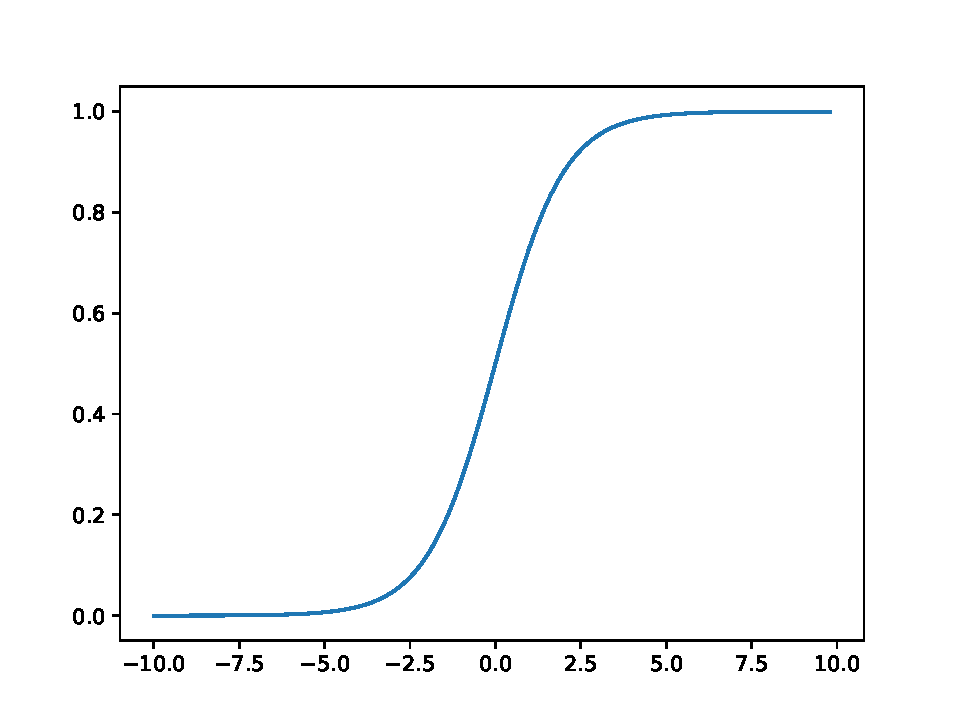
\includegraphics[scale = 0.7]{figures/machineLearning/sigmoid.pdf}
                \caption{Sigmoid function, as can be seen it outputs a value between 0 and 1, $h_\theta(x) \geq 0.5$ is classified as $1$, $h_\theta(x) < 0.5$ is classified as $0$}
                \label{fig:sigmoid}
            \end{figure}
            
            
            
            % \begin{align}
            %     err(h_\theta(X),y) = 
            %     \begin{cases}
            %         1 &\text{if } h_\theta(X),y) \geq 0.5 \text{ and } y = 0 \text{ or } h_\theta(X),y) < 0.5 \text{ and } y = 1 \\
            %         0 &\text{else}
            %     \end{cases}
            % \end{align}
            
    
            
        
            \subsubsection{Support vector machines}
            
            Support vector machine or SVM, can be used for both supervised and unsupervised learning. In the unsupervised case, it is most commonly used for outlier and boundary detection. For supervised learning it handles two classes at a time, so one vs the rest is used if there are more than two classes. The classifier defines a hyperplane that separates the two different classes. The hyperplane can then later be used to predict which class a new feature vector belongs to.  
            
            In general SVM follows the same patterns as the regression classifiers explained above. A cost function is minimized by finding the gradient of it, and the parameters are updated accordingly. Either to convergence or until a given number of iterations are reached. 
            
            SVM is capable of separating data both linearly and nonlinearly. How the algorithm separates the data depends on the kernel function it uses. A kernel function, or a similarity function, describes how similar two feature vectors are by taking the inner product of the two samples in a higher dimensional space. The kernel function does this without having to explicitly transform the data into this dimension. This means that nonlinear shapes can be detected without having to explicitly calculate the new feature space, as is the case with linear and logistic regression. 
            
            A hyperplane is a plane that has one less dimension than the original feature space. So for a two dimensional feature space, the hyperplane becomes a line. By this logic one should not be able to define a complex nonlinear decision boundary for the 2D feature space, but here is where the kernel trick comes to the rescue. 
            
            If the Gaussian kernel
            
            \begin{align}
                K_g(\bm x^{1},\bm x^{2}) = e^{\frac{\norm{\bm x^{1}-\bm x^{2}}^2}{2\sigma^2}} 
                \label{svm:gauss}
            \end{align}
            
            is used, each datapoint in the 2D feature space is transformed into 3D. The third dimension now becomes the evaluation of the kernel function. Hence the hyperplane that now separates the two classes becomes a 2D plane. The choice of $\sigma$ for the Gaussian kernel is important when looking into over- and underfitting. 
            
            The polynomial kernel,
            \begin{align}
                K_p(\bm x^{1},\bm x^{2}) = (\bm x^{1T}\bm x^{2} + \alpha)^\beta,
                \label{svm:poly}
            \end{align}
            
            is another example of a kernel function. Here $\beta$ correspond to the polynomial degree and $\alpha$ is a bias term. These are just two of many examples. The Gaussian or RBF kernell is a good first choice if you know that you have a nonlinear boundary, but don't know exactly what shape the boundary will take. If you have more knowledge about the shape of the boundary you are looking for, you might want to consider more special kernels.
            
            The following mathematical derivation is based on \cite{Hastie}, and a more thorough explanation can be found in its chapters 4.5 and 12. The main goal is to give the reader an intuition on how the algorithm works. 
            
            \begin{align}
                f(\bm x) = \beta_0 + \bm \beta^T\bm x = 0,
                \label{svm:hyper}
            \end{align}
            
            
            defines a hyperplane. For any two feature vectors $\bm x^{[1]},\bm x^{[2]}$ that lie in or on the hyperplane where $\bm \hat x = \bm x^{[1]} - \bm x^{[2]}$, gives  $\bm \beta^T \bm \hat x = 0 $ and hence, $\bm \beta$ is a scalar multiplication of the normal vector to the hyperplane, 
            
            
            \begin{align}
                \bm \beta^* = \frac{\bm \beta}{\norm{\bm \beta}}.
                \label{svm:norm}
            \end{align}
            
             When inserting any feature point $\bm x_0$ that lies on or in the hyperplane defined by Equation \ref{svm:hyper}, one get $\bm \beta_0 + \bm \beta^T\bm x_0 = 0$ which yields $\bm \beta^T\bm x_0 = -\bm \beta_0$. 
            
            
            
            By using $\bm x_0$ as any feature vector from origo to the hyperplane and the normal vector $\bm \beta^*$, the distance for any given feature vector $\bm x$ to the hyperplane is given by
            
            \begin{align}
                \bm \beta^{*T}(\bm x - \bm x_0) = & \frac{\bm \beta^T}{\norm{\bm \beta}} (\bm x - \bm x_0) \nonumber \\
                = & \frac{1}{\norm{\bm \beta}}(\bm \beta^T\bm x- \bm \beta^T\bm x_0) \nonumber \\
                = & \frac{1}{\norm{\bm \beta}}(\bm \beta^T\bm x + \bm \beta_0) \nonumber \\
                = & \frac{1}{\norm{f'(\bm x)}}f(\bm x).
                \label{svm:dist}
            \end{align}
            
            
            
            A decision rule 
            
            \begin{align}
                y^i(\bm x^{iT} \bm \beta + \beta_0) \geq 1 
                \label{svm:decision}
            \end{align}
            
            can then be created using the hyperplane. Since there are two classes they are defined as $y_0 = 1$ and $y_1 = -1$. The decision rule tells which class a feature vector belongs to.
            
            
            
            
            
            Now that an expression for the distance from a hyperplane to any given feature vector in the feature space is defined, one can look at how to find the optimal hyperplane to separate the two classes. The margin or the width between the two closest point from both classes can be defined as $M = \frac{2}{\norm{\bm \beta}}$, and hence maximizing the distance can be formulated as minimizing 
            
            \begin{align}
                J(\bm \beta) = & \frac{1}{2}\norm{\bm \beta}^2 \nonumber \\
                 s.t \quad y^i(\bm \beta^T\bm x^i + \beta_0) \geq & 1 \quad \forall \enspace i.
                \label{svm:cost}
            \end{align}
            
            The constraint here ensures that every point is classified correctly.
            
            \begin{align}
                L = \frac{1}{2}\norm{\bm \beta}^2 - \sum_{i=1}^n \alpha_i[y^i(\bm \beta^T\bm x^i + \beta_0) - 1]
                \label{svm:lagrange}
            \end{align}
            
            shows the equation rewritten as a Lagrangian optimization problem. Setting the partial derivative of $L = 0$, gives the expression

            \begin{align}
                \frac{\partial L}{\partial \bm \beta} = & \bm \beta - \sum_{i=1}^n \alpha_i y^i\bm x^i \nonumber\\
                \bm \beta = & \sum_{i=1}^n \alpha_i y^i\bm x^i, 
                \label{svm:partialbeta}
            \end{align}
            and
            
            \begin{align}
                \frac{\partial L}{\partial \beta_0} =& -\sum_{i=1}^n \alpha_i y^i \nonumber   \\
                \sum_{i=1}^n \alpha_i y^i =& 0
                \label{svm:partialbeta0}
            \end{align}
            
            Inserting Equation \ref{svm:partialbeta} and \ref{svm:partialbeta0} into \ref{svm:lagrange}, gives the Wolfe dual maximization problem,
            
            \begin{align}
                L = \sum_{i=1}^n  \alpha_i - \frac{1}{2} \sum_{i=1}^n \sum_{j=1}^n \alpha_i \alpha_j y^i y^j \bm x^{iT} \bm x^j.
                \label{svm:dual}
            \end{align}
            
            One of the great benefits of the SVM is that the Lagrangian optimization problem defined in Equation \ref{svm:dual} is a convex optimization problem, and hence it has a global maxima.
            
            
            If your classes are not linearly separable in the feature space, maximization of Equation \ref{svm:dual} has no global solution. However as can be seen in Equation \ref{svm:dual} one want to minimize $\bm x_i^T  \bm x_j$. This term can then be replaced by the kernel function defined in paragraph three in this section, which now enables separation in a higher dimensional space.
            
            
            
            
            One interesting observation can be made by inserting Equation \ref{svm:partialbeta} into Equation \ref{svm:decision}. This yields 
            
            \begin{align}
                y^i(\sum_{j=1}^n \alpha_j y^j \bm x^{iT}\bm x^j + \beta_0).
                \label{svm:decision2}    
            \end{align}
            
            Both the decision function and the optimization problem depend only on the pairs of dot product of the x vectors. Which further supports the usage of the kernel functions. The final thing to remark is that not all datasets are completely separable, to deal with this a slack variable is introduced into the optimization to allow miss-classification of some of the feature vectors. 

    
            \subsubsection{Neural networks}
            A neural network attempts to make a machine learn like humans. The algorithm is modeled from how we think the neurons in the human brain learn. A fascinating fact is that a four year old child is better at classifying images than a modern supercomputer. If one could Figure out exactly how the human brain works, and implement a similar learning scheme for computers, only the sky would be the limit. A NN can be look at as an extension of the regression methods described above. In the regression methods the input data $\bm x$ is given to a function $h_\theta(\bm x)$, that either predicts a continuous value, or a class. In a NN, instead of letting $h_{\theta}(\bm x)$ serve as the prediction, the output is used as input for a new layer.
            
            \begin{figure}[h]
                \centering
                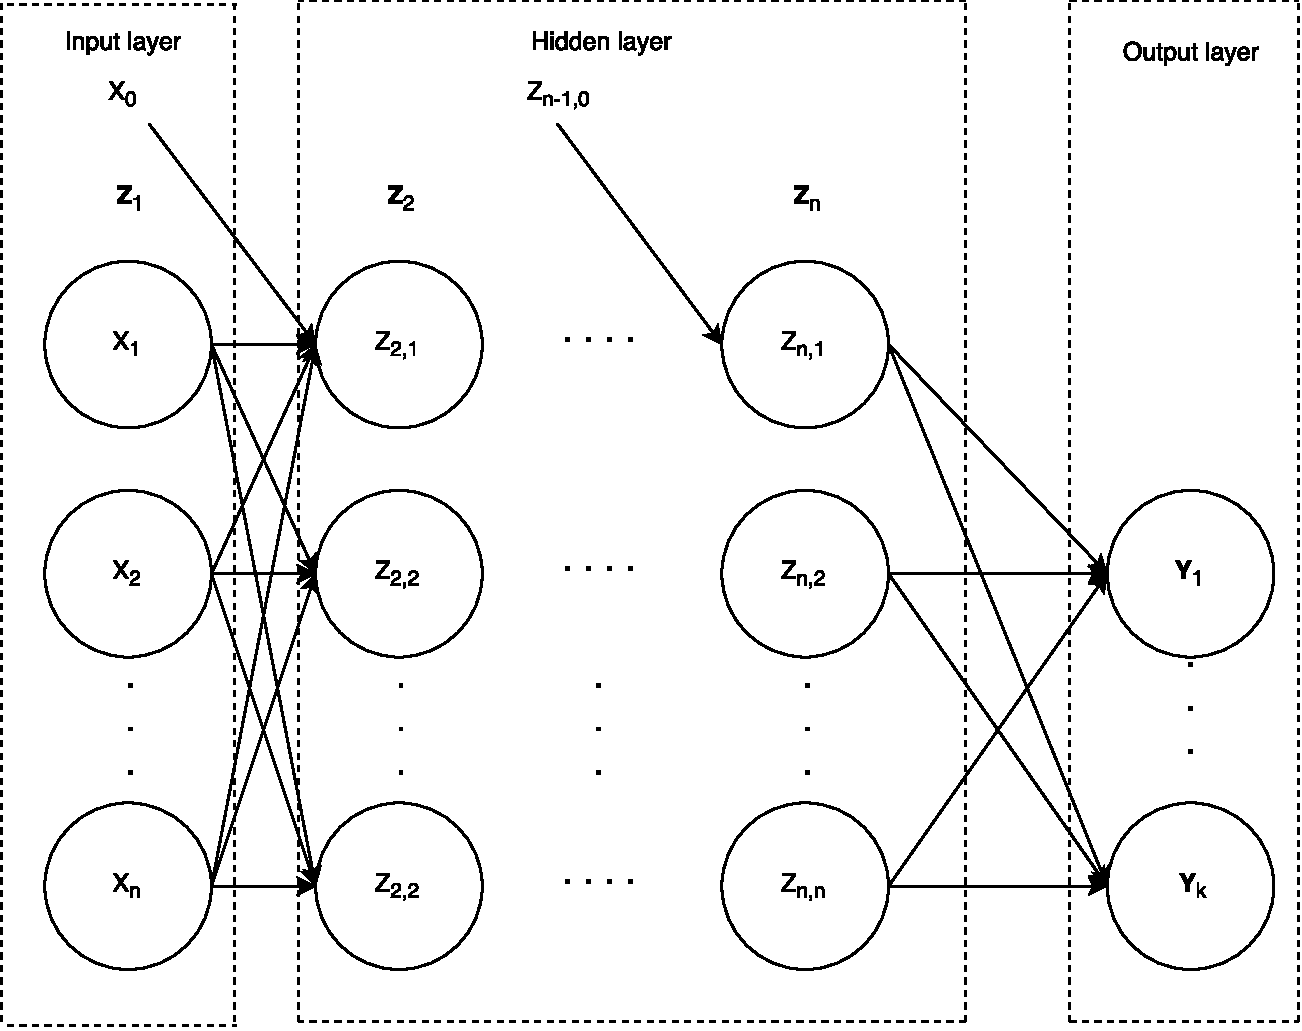
\includegraphics[width=0.8\textwidth]{figures/machineLearning/neural_network.pdf}
                \caption{A graph visualizing a N-level deep neural network}
                \label{fig:nn_fullnetwork}
            \end{figure}
            
            
            
            A NN is a n class classification or regression algorithm. A good visual representation is a graph with nodes and vertices as shown in Figure \ref{fig:nn_fullnetwork}. As seen, a NN consist of three parts. An input layer, a hidden layer and an output layer. The input layer is the feature vectors for the data samples, the hidden layer does all the computation and the output layer does the prediction. A NN with only one layer and a limited number of neurons, can approximate any function \cite{Hastie}. This shows how power full a NN can be. Notice that in Figure \ref{fig:nn_fullnetwork} a bias feature is added to every layer, that is not a part of the original feature set. A NN used for regression, will normally have $k=1$ for the output layer, while a NN for classification will have $k=\textit{\#classes}$. Even if a NN is capable of approximating any function, it does not necessarily mean that it is a trivial task. The more nodes and layers a NN consists of, the harder the network become to interpret. Note that Figure \ref{fig:nn_fullnetwork} have all the outputs from the previous layer, connected to all neurons in the next layer, this is not necessarily the case.
            
            
            \begin{figure}[h]
                \centering
                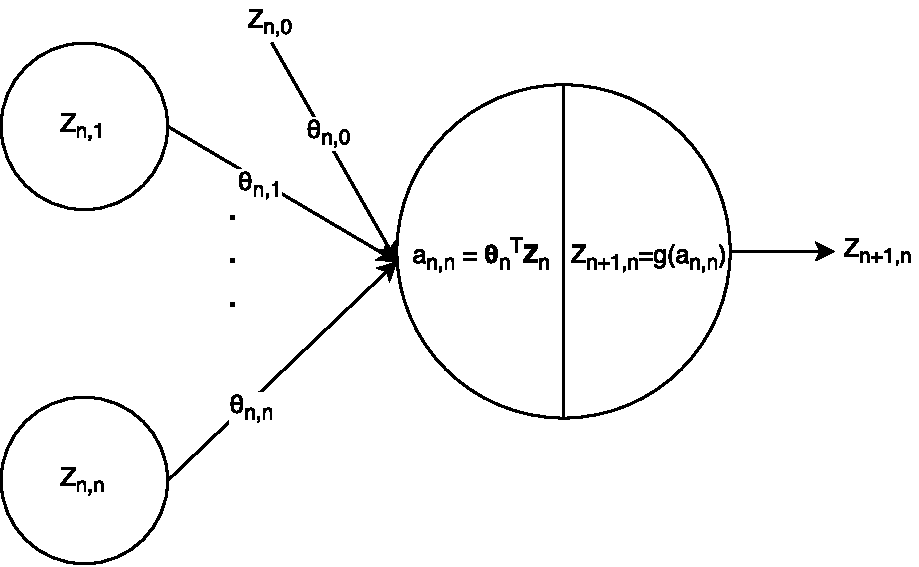
\includegraphics[width=0.5\textwidth]{figures/machineLearning/single_neuron.pdf}
                \caption{Visualization of a single neuron}
                \label{fig:nn_neuron}
            \end{figure}
            
            The following mathematical derivation is based on \cite{Hastie}, \cite{Ng}, and \cite{Nga}. Each of the nodes marked  $z_{n,n}$ seen in Figure \ref{fig:nn_fullnetwork} is what we call a neuron. A single neuron is visualized in Figure \ref{fig:nn_neuron}. Each neuron does two things. First it takes the dot product of the input vector and the weight vector, 
            
            \begin{equation}
                a = \bm \theta_n^T \bm Z_n,
                \label{eq:neuron_a}
            \end{equation}
            
            also shown in Figure \ref{fig:nn_neuron}. Then the output $Z_{n+1,n}$ is calculated 
            
            \begin{equation}
                Z_{n+1,n} = g(a_{n,n}).
                \label{eq:nn_activation}
            \end{equation}
            
            Here $g(a)$ is known as an activation function. There are many different options for activation functions, the most common are shown in Table \ref{tab:acitvations}. If the identity function is used, one can easily verify from Figure \ref{fig:nn_neuron} that a one layer NN is actually the same as regression. When working with classification, the most commonly used activation functions are Relu and Sigmoid/Softmax. All of these functions are nonlinear, and it is by using nonlinear activation functions, that a NN is enabled to approximate any function. If only linear functions are used, it can be verified that adding more layers does not but complicating a linear interpretation \cite{Hastie}. 
            
            
            %%%%%%%%% activation fucntions 
            % \begin{align}
            %     g_k(a) = a \textit{ identity function} \\
            %     g_k(a) = \frac{1}{1+e^{-a}} \textit{ sigmoid function} \\
            %     g_{k}(a) = \frac{e^{Tk}}{\sum_{i=1}^Ke^{Ti}} \textit{ softmax function} \\
            %     g_{k}(a) = \frac{e^a-e^{-a}}{e^a+e^{-a}} \textit{ tanh function} \\
            %     g_{k}(a) = max(a,0) \textit{ relu function}
            %     \label{eg:activations}
            % \end{align}
            
        \begin{table}[h]
            \centering
            \begin{tabular}{ | c | c |}
                \hline
                Function & Function\\ \hline
                Identity & $g_k(a) =a$ \\ \hline
                Sigmoid & $g_k(a) =\frac{1}{1+e^{-a}}$ \\ \hline
                Softmax & $g_k(a) =\frac{e^{Tk}}{\sum_{i=1}^Ke^{Ti}}$ \\ \hline
                Tanh & $g_k(a) =\frac{e^a-e^{-a}}{e^a+e^{-a}}$ \\ \hline
                Relu & $g_k(a) =max(a,0)$ \\ \hline
            \end{tabular}
            \caption{Different activation functions}
            \label{tab:acitvations}
        \end{table}
                    
            % \begin{align}
            %     z_{m} =  \sigma(\theta_{0m} + \bm \theta_m^T \bm z_{m-1}), \textit{m = 1,..,M} \nonumber \\
            %     \bm \hat y = g(\bm z_m) \nonumber \\
            %     \label{eq:fwdprop} 
            %     % \textit{where $\sigma()$ and g() are different activation function}\nonumber 
            % \end{align}
            % In the first layer, $\bm z_1 = \bm x$. For all the other layers each $z_m$ is given by the activations function of a bias term pluss the dot product of the inputs $\bm z$ and the weight $\bm \theta$. This means that for each layer there exists $m$ $\bm \theta$ vectors, which can be written as $\bm \Theta_m$. For the regression classifiers one only had one vector $\bm \theta$, but for a NN you end up with $m$ $\bm \Theta$ matrices. This gives a good indication on why a NN can approximate any given function. 
            
            In the final layer, the output $\hat y$ is calculated. The number of elements in the final layer depends as mentioned if classification or regression is being performed. For regression, the final layer normally only has one element, but for classification, it holds as many elements as there are classes. For binary classification, the Sigmoid function is normally used. For k-class classification, the Softmax function is used, and for regression the identity function. 
            
            
            
            The iteration through the NN mentioned above, is known as forward propagation. It takes a feature vector as input, process it through the layers and either predicts a class or a value. But this does not explain how the NN is trained. As with the regression methods, the weight or coefficients in $\bm \Theta = [\bm \Theta_1 ... \bm \Theta_n]$ needs  to be updated.  This update step is known as backpropagation. The goal is to minimize a cost function as a function of $\bm \Theta$. The cost function used in a NN depends on whether or not it is regression, binary or k-class classification. The three different options are 
            
            \begin{align}
                E(\bm\Theta) = &\sum_{i=1}^M\frac{1}{2}(\hat{y} - y)^2 \nonumber\\
                E(\bm\Theta) = & -\sum_{i=1}^M(y\log(\hat{y})+(1-y)\log(1-\hat{y}) \nonumber\\
                E(\bm\Theta) = &- \sum_{i=1}^m \sum_{k=1}^K y_{ik}\log(\hat y),
                \label{nn:cost}
            \end{align}
            
            
            for a training set of size M. For k-class classification the inner summation is over all the classes. It is not only important to verify that the correct class is predicted, it is equally important that not any of the other classes are wrongly predicted.
            
            
            
            
            The same approach is used for minimizing $E(\bm \Theta)$ as for the previous methods. Gradient descent or another optimization algorithm is used to calculate each of the different parameters in $\bm \Theta$'s contribution to the cost. $\bm \Theta$ is updated as 
            
            \begin{align}
                \bm \Theta := & \bm \Theta - \alpha \nabla E(\bm \Theta) \nonumber \\
                \Theta_{ij} = & \Theta_{ij} - \alpha \sum_{k=1}^M \frac{\partial E_k}{\partial \Theta_{ij}} 
                \label{bp:1}
            \end{align}
            
            Here $\alpha$ is the learning rate, as described in a previous section. As can be verified by the equations in \ref{nn:cost}, the total cost increases when a prediction does not match the given label.
            
            
            The intuitive explanation to what the backpropagation does, is that the prediction errors, can be back-propagated to calculate the error in each neurons prediction. This prediction error is then used to update the corresponding weights for the neuron in matrix $\bm \Theta$. The partial derivative of the cost function is defined as
            
            % Equation \ref{bp:1} to \ref{bp:9} shows how the partial derivative of the cost function is computed.   
            
            \begin{align}
                \frac{\partial E}{\partial \Theta_{ji}} = \frac{\partial E}{\partial a_{ji}} \frac{\partial a_{ji}}{\partial \Theta_{ji}} \label{bp:2}.
            \end{align}
            
            Solving for the first term,
            \begin{align}
                \delta_{ji} \coloneqq \frac{\partial E}{\partial a_{j,i}} = \sum_{k=1}^N \frac{\partial E}{\partial a_{j+1,k}} \frac{\partial a_{j+1,k}}{\partial a_{ji}} \label{bp:3}
            \end{align}
            
            where
            
            \begin{align}
                 \frac{\partial E}{\partial a_{j+1,k}} = \delta_{j+1,k}
            \end{align}
            
            and
            \begin{align}
                \frac{\partial a_{j+1,k}}{\partial a_{ji}} = \frac{\partial \bm \theta_{j+1}^T \bm Z_{j+1}}{\partial a_{ji}}. \label{bp:4}
            \end{align}
            
            $\bm \theta_{j+1}^T \bm Z_{j+1}$ can be written as, 
            
            \begin{align*}
                \bm \theta_{j+1}^T \bm Z_{j+1} = \Theta_{j+1,0}Z_{j+1,0} +\textit{ }..+ \textit{ }\Theta_{j+1,N}Z_{j+1,N} \nonumber \\
                = \Theta_{j+1,0}g(a_{j,0}) + \textit{ }.. +\textit{ }\Theta_{j+1,N}g(a_{j,N}). \label{bp:5}
            \end{align*}
            
            This gives, 
            \begin{align}
                \frac{\partial a_{j+1,k}}{\partial a_{ji}} = \Theta_{j+1,i}\frac{\partial g(a_{j,i})}{\partial a_{ji}} =  \Theta_{j+1,i}g'(a_{ji}), \label{bp:6} 
            \end{align}
            
            which finally yields
            \begin{align}
                \delta_{ji} = g'(a_{ji})\sum_{k=1}^N\delta_{j+1,k}\Theta_{j,k}. \label{bp:7}
            \end{align}                    
            
            Solving for the second term
            \begin{align}
                a_{ji} = \bm \theta^T_i \bm Z_{i} \label{bp:10}
            \end{align}
            
            \begin{align}
                \frac{\partial a_{ji}}{\partial \Theta_{ij}} =  Z_{ji} \label{bp:8}
            \end{align}
            
            Gives the following equation
            \begin{align}
                \frac{\partial E}{\partial \Theta_{ji}} = \delta_{ji}Z_{ji} \label{bp:9}
            \end{align}
            
            
            
            
            The forward and backwardpropagation steps are then iterated over until a given number of iterations are reached. A complete pass forward and backward of all training examples, is known as one epoch. When the training set is large, it is often split into smaller batches to speed up calculations. The batch size tells you how many samples should be included in each forward and backward pass. Splitting the data into batches enables the algorithm to take advantage of parallelism, running the separate batches on separate CPU's or GPU's. Notice in Equation \ref{bp:9} that $Z_{ji}$ is a part of the expression. This term is calculated as a part of the forward propagation, hence when developing a NN storing these values will reduce the computation time. 
    
                
            When you design a NN, you are free to make it as wide and deep as you want. However, the deeper you make it, the more processing each iteration through it will take. Deep networks also increases the risk of overfitting. A good approach is to start with a shallow network, and increase the depth and width until you see that adding new layers, does not yield better performance. To avoid overfitting the regularization term 
            
            \begin{align}
                \frac{\lambda}{2} \sum_{km} \Theta_{km}^2  \nonumber \\
                = \frac{\lambda}{2}\bm \Theta^T \bm \Theta,
                \label{nn:overfit}
            \end{align} 
            
            is added to the cost function. The extra term in the cost function will penalize parameters $\neq 0$.   
            
            
            This slightly modifies the update rule as 
            
            \begin{align}
                \bm \Theta = & \bm \Theta - \alpha \nabla E(\bm \Theta) - \alpha \frac{\lambda}{2} \frac{\partial \bm \Theta^T \bm \Theta}{\partial \bm \Theta} \nonumber \\
                = &(1-\alpha \lambda)\bm \Theta - \alpha \frac{\partial E(\bm \Theta)}{\partial \bm \Theta}.
                \label{nn:updaterule2}
            \end{align}
            
            Since the regularization term is introduced to reduce the weights in the NN, it is a natural conclusion that the weights should be initialized to small values. Zero initialization is however not a good option, this will lead to zero derivatives, and hence the model will never be updated. Initializing all weights to a random number near zero, will give a roughly linear model \cite{Hastie}. This means that the model will start out more or less as a linear function and will grown in nonlinearity if necessary. 

    \subsection{Scikit-learn}
    Scikit-learn \cite{scikit-learn}, \cite{scikit-web} is an open source toolbox available for Python. It includes a number of different machine learning algorithms and the tools needed to preprocess and analyze your data. The framework created by scikit-learn is used throughout this project, mainly because it either includes the algorithms that are to be tested, or there exist an API that allows you to run the non existing algorithms through the scikit-learn framework. 
    
    In addition to the being a great machine learning library for Python, the website \footnote{\url{http://scikit-learn.org/stable/ }}also explains the main theory behind the different algorithms, and what the scikit-learn algorithms are built upon in a easy to find manner. This makes it a good choice when one want to understand what is making the algorithms work.        
    
    \subsection{Keras}
        Scikit-learn does not include neural networks. Different libraries were considered before Keras was chosen for the NN analysis. Keras \cite{chollet2015keras} is a Python library that simplifies creation of NNs in Python. Instead of having its own implementation of NNs, it uses other NN python libraries as backends. This means that you can run you analyzis using for example Google's TensorFlow through Keras. At this moment Keras supports Google's TensorFlow, Theano developed by LISA Lab at Université de Montréal and CNTK developed by Microsoft. This means that by using Keras, only one line of code needs to be changed if one want to change between one of the options above. Developing code using one of the NN libraries directly would make switching between the different options more cumbersome. However, one important factor to keep in mind, is that Keras is not officially supported by any of the backend developers. This means that  not all of the original functionality is guaranteed to be supported in Keras. Regardless, the fact that Keras is easy to use and its focus on enabling fast experimentation, are the main reasons for developing in Keras. Keras supports the normal sequential NN which is used in this analysis, but it also has support for the more complex convolutional and reccurent NN. It can also run on both CPU and GPU, making it flexible and optimizable to the hardware it runs on. More information about Keras can be found at \footnote{\url{https://keras.io/}}.
            
        \subsubsection{Google TensorFlow}
            For this project only the TensorFlow backend is tested. TensorFlow \cite{Abadi} is developed by The Google Brain project, and it started as the DistBelif project back in 2011. Tensor flow is the second generation, built upon the experiences from DistBelif. Tensorflow has support for parallelism and has the possibility to have many different devices collaborating on the same problem. As stated in \cite{Abadi}, "a computation expressed using TensorFlow can be executed with little or no change on a wide variety of heterogeneous systems, ranging from mobile devices such as phones and tablets up to large-scale distributed systems of hundreds of machines and thousands of computational devices such as GPU cards". This shows the flexibilty TensorFlow introduces. More information about TensorFlow can be found at \footnote{\url{https://www.tensorflow.org/}}.
        
        
        
    % \subsection{Evalutation of the classifiers}
    
    %     \subsubsection{F1 score}
    %     \subsubsection{accuracy}
    %     \subsubsection{Learning curves}
    %     \subsection{Visual checking}
        
        
        
    \subsection{How the different algorithms are analyzed}
        \subsubsection{Prediction accuracy}
            One way to evaluate the classifiers performance is using the prediction error. An error function for a two class classifier is defined as
            
            \begin{align}
                \err(h_\theta(X),y) = 
                \begin{cases}
                    1 &\text{if } h_\theta(X),y) \geq 0.5 \text{ and } y = 0 \text{ or } h_\theta(X),y) < 0.5 \text{ and } y = 1. \\
                    0 &\text{else}.
                \end{cases}
                \label{eq:error_func}
            \end{align}
            As can be seen, a prediction is classified as wrong if rounding it to the nearest integer $(0,1)$ gives a different value than the data label given by the label set. The test error is then calculated by summing over all pairs $\bm{x_{train}^i}, y_{train}^i$ and calculating the average value by dividing by the number of samples, 
            \begin{align}
                \frac{1}{m} \sum_{i=1}^{m_{test}}\err(h_\theta(x_{test}^i,y_{test}^i).     
                \label{lr:testError}
            \end{align}
            This is used to classify the different logistic regression classifiers, and to pick the best one. One need to take caution when applying a test like this on skewed datasets. If the data set is very skewed, with only a small number of for example negative training examples, then a classifier that predicts $1$ for all data-points will score well on the test error, even if it predicts every negative training example wrong. 
            
            
        \subsubsection{F1 score}
            Prediction error or prediction accuracy are a quick ways to look at your classifiers performance. However, high accuracy does not necessarily mean that your classifier is doing a great job. To deal with the skew issue F1 score is introduced. The F1 score is calculated as
            
            \begin{align}
                F1 = 2\frac{\text{precision}*\text{recall}}{precision+recall}.
                \label{eq:f1_score}
            \end{align}
            
            For this to make sense, the terms precision, 
            
            \begin{align}
                \text{Precision} = \frac{\text{\#TruePositive}}{\text{\#TruePositive}+\text{\#FalsePositive}},
                \label{eq:precision}
            \end{align}
            and recall,
            \begin{align}
                \text{Recall} = \frac{\text{\#TruePositive}}{\text{\#TruePositive}+\text{\#FalseNegative}},
                \label{eq:recall}
            \end{align}
            
            needs to be explained. Equation \ref{eq:precision} and \ref{eq:recall} show how the two different terms are computed, and Table \ref{tab:prerec} explains the different terms
            
            \begin{table}[h]
                \centering
                \begin{tabular}{| p{4cm} | p{4cm} |}
                    \hline
                    Term & Explanation\\ \hline
                    \#TruePositive & The number of predictions classified to the class correctly.\\ \hline
                    \#FalsePositive & The number of predictions classified to the class wrongly. \\ \hline
                    \#FalseNegative & The number of predictions that should have been classified to the class, but are not. \\ \hline
                \end{tabular}
                \caption{Explanation of the terms used to calculate the $F1$ score}
                \label{tab:prerec}
            \end{table}
            
            Hence one should calculate the $F1$ score for all classes, to check a classifiers performance. 
        
        % \subsubsection{Precision recall curve}
        %     To get av more visual representation of the performance on skewed datasets, precision/recall curves can be used. 
        %     Once plotted the graph shows how well the prediction has gone by the area under the curve. The larger the area, the better the performance. create plots for the different lr classifiers, to confirm that performance is increasing until degree 8.
        %     Use the curve to show if it is precision or recall that is large for the F1 score. Since the F1 score is already beeing used to numerically evaluate the performance. 
        
        \subsubsection{Learning curves, bias vs variance}
            The $F1$ score tells you how well your classifier is doing. However, it does not tell you what you should do if it is not yielding sufficient results. This is where learning curves, bias and variance comes into play. A learning curve plots the classifiers performance  on the training and cross validation set, as a function of the training set size. In it simplest form, you split your data into two parts traning and test sets. At first you only use a small subset of the training set to train your classifier. After training you check your classifiers performance on the subset used for training, and also on the test set. The size of the traning set is then increased for each iteration to see if more data yields a better performance. Figure \ref{fig:learning_curves} shows what a learning curve plot can look like. As can be seen the accuracy on both training and test set increase as the number of training samples increases. One important thing to notice is that both training and test predictions follow each other very closely. This is indicates that the test set is not holding much new information compared to the training set, hence the better the algorithm fits the training set, the better it fits the test set.  
            
            \begin{figure}[h]
                \centering
                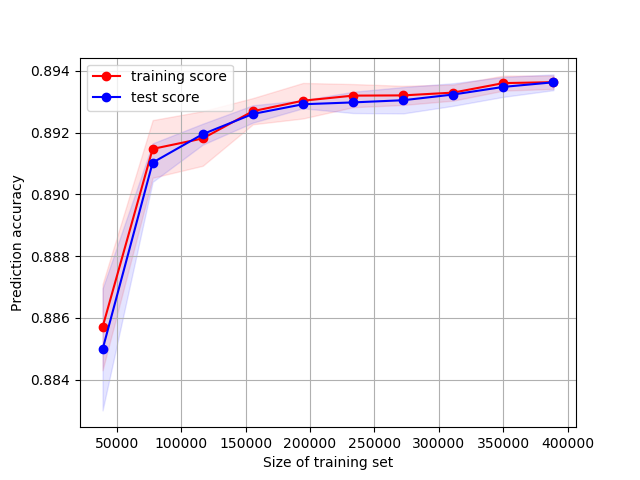
\includegraphics[scale = 0.8]{figures/machineLearning/LearningCurves.png}
                \caption{Learning curve showing the accuracy of the prediction on both test and training sets, as a function of growing training set size}
                \label{fig:learning_curves}
            \end{figure}
            
            Bias and variance are two terms used to describe whether or not the trained classifier is underfitting or overfitting the data model. Underfitting occurs when you try to adapt a too simple model to your data. A good example is trying to fit a line to a circle. No matter how large your training set is, you will never be able to get a good fit between the model and the data. This is known as high bias, and the solution is to use a more complex model. High bias will often give poor predictions on both training and test sets. Variance is on the opposite side, high variance means that you are overfitting the data. No real life dataset is perfect, and by using a too complex model or by not having enough training data this can become an issue. High variance can often be confirmed with a much better training prediction accuracy than test prediction accuracy.  

        \subsubsection{Finding the best parameters for your classifier}
            When you are using one of the ML algorithms to create a classifier, there is a number of parameters you can set, to adjust how the algorithm perform. This is known as hyperparameterization. The basic way to do it, is to create a number of classifiers for the different combinations of input parameters, and to split your dataset into a training and cross validation set. You then use the prediction accuracy on the cross validation set, to determine which of the parameter combinations that yields the best result. To implement this yourself, is however a cumbersome thing, and it would take a lot of time. In this project, a built in method from the scikit-learn library is used instead. 
            
            There are two main approaches, Grid Seach and Randomized search. In most cases Grid Search is performed as an exhaustive search, meaning that it checks all possible combinations of the hyperparameters, to find the best fit. Randomized search, randomly picks a a subset of the parameters for n given iterations, and the best ones are kept. This will drasticly reduce computation time when the number of parameters are large. According to \cite{BergstraJAMESBERGSTRA2012} randomized search performs as well as grid search when the number of parameters grows large, and does so in a much faster manner. Therefor the latter is used.
            
        
        
    % \subsection{PyTorch?}
    %     PyTorch is an alternative to Tensorflow when you want to use neural networks for deep learning. It is a relatively new framework, but is beeing developed fast. Many experts also claim that Pythorch will exist alongside Tensorflow for a long time. Pytorh

    
    
    % \subsection{Preprocessing of data}
    %     The dataset used in this project, has a lot of common data areas. As mentioned, the goal is to enable prediction of a servo indicator's state, based on process signals. The datasets are extremely large, but many of the datapoints does not include any new information, they are simply overlapping other data points, or are from a data set which all servo indicators can generate independent of their current state. Hence one can argue that it would be beneficial to remove those data points to simplify the data analysis. 
        
    %     Need to show plots of the data sets, and explain why this actually is a fact. 
        
    %     \subsubsection{Feature Scaling}
        
    %     \subsubsection{Mean normalization}
        
            
        
    %     \subsubsection{Load reduction}
    %         This section is intended to explain why some of the data points in the data sets are complicating the analysis without adding more information. The power output of the hydro electric power station is controlled by the power consumption of the grid. Increase or decrease in power production is controlled by controlling the flow of water into the turbine, this is again controlled by the servo indicators. When the $\Delta P$ is large enough, this means that $\Delta Flow$ need to change accordingly. When the servo indicators change from steady state to closing or opening, you get hysteresis, which can be seen in the figure. The issue with the data points that are sampled during this hysterisis is that they are common for all servoindicators, both new and old. Hence you are not able to directly observe wether or not the data point should belong to one class or the other. Of course there might be information hidden in the data that you cannot observe in the figures, that can be picked up by a deep neural network. Therfore the emphasis in this project is to check performance between heavily preprossed data, and simple classifiers vs scaled raw data using deep neural networks. 
            
    %     \subsubsection{Median filter}
    %         The first filter used to remove datapoints which fall into the above category is median filter. As can be seen in the figure, it also removes datapoints not related to a change of direction, but it significantly removes the data points in focus, and also reducec the number of data points in the data set. 
            
    %         The median filter is a rolling filter. As the name implies it uses the median of a data set. The clue here is that it takes the median of a given window of the total data set at a time. This enables you to find the median for a subset of the data, calculate the median, and remove outliers, hence datapoints that have a large rate of change. 
            
    % \subsection{Hyperparameter optimization}
        
        
        
    % \subsection{Classifier evalutation}
    
    %     As can be seen, a prediction is classified as wrong if rounding it to the nearest integer $(0,1)$ gives a different value than the data label given by the label set. The test error is then calculated by summing over all pairs $x_{train}^i, y_{train}^i$ and calculating the average value by dividing by the number of samples as can be seen in \ref{lr:testError}. 
    %         \begin{align}
    %             \frac{1}{m} \sum_{i=1}^{m_{test}}err(h_\theta(x_{test}^i,y_{test}^i)     
    %             \label{lr:testError}
    %         \end{align}
    %     This is used to classify the different logistic regression classifiers, and to pick the best one. One need to take caution when applying a test like this on skewed datasets. For the datasets used here, there are the same number of negative and positive training examples. This is done by only picking the same amount from both sets of data. If you however have a very skewed data set, with only a small number of for example negative training examples, then a classifier that predicts $1$ for all datapoint will score well on the test error, even if it predicts every negative training example wrong. 
        